\chapter{Summary}
Here, I will review the findings from the previous sections. I will consider the implications of AI in this paper regarding its performance compared to a human playing a game. I will also include a discussion of any lessons learned from the project and any future work that can be done.

\section{The game development}
The progress of the game took most of the time due to the lack of sources in the PyGame library with the right functions that I was looking for then. Generating the function was the part that took most of the time. I remember that I spent more than a month trying to figure out a way to make the wave have a random amplitude so the player wouldn't cheat in the game. The problem was finding a way to make the wave one sequence after generating with the new amplitude, as it would shift the new sequence by a specific amount of pixels on the x-axis, either positively or negatively, in relation to the last point in the old sequence.
\begin{figure}[H]
	\centering
	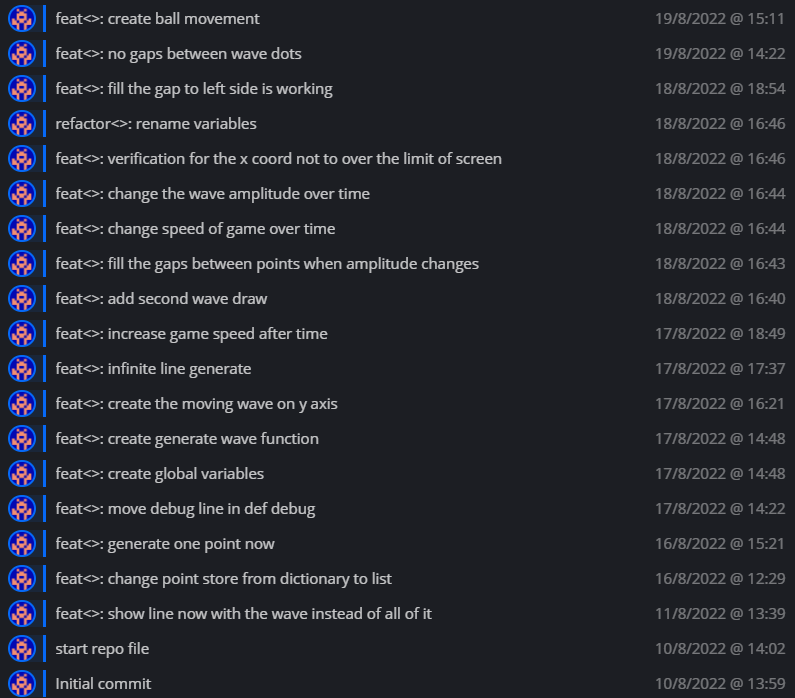
\includegraphics[width=0.7\linewidth]{usedImages/repoStart}
	\caption[]{the start of game repository on GitHub}
	\label{fig:repostart}
\end{figure}

Dealing with the other parts, such as, making the game follow the principle of encapsulation, took more than 3 days of continued work. Something I had before was the problem of having one file that did the functionality for all components of the game. For instance, the reset function that existed in ball functions is responsible for resetting the whole game, including wave-related variables. It is preferable to create a class for the wave and then include a function in it to reset the associated variables. You can call the wave functions whenever you want.

In my opinion, this is preferable, because I would be confused about which variables to call and would benefit from a better file management for each component of the game. 
\begin{figure}[H]
	\centering
	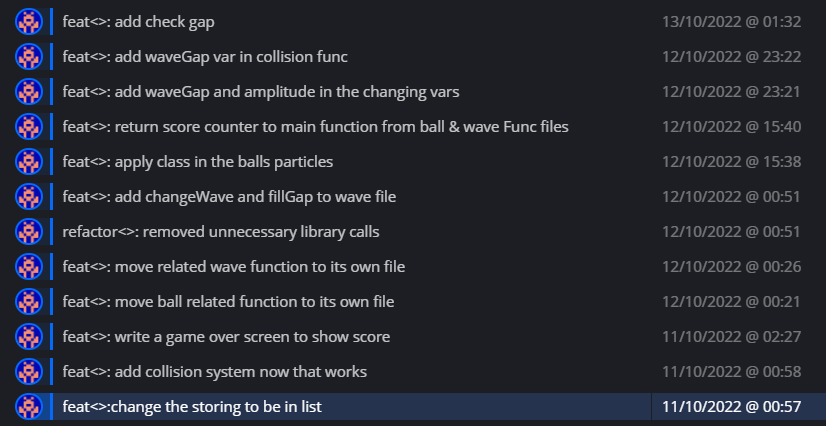
\includegraphics[width=0.7\linewidth]{usedImages/repoEncapsulation}
	\caption[]{Time it took to implement the new layout in encapsulation}
	\label{fig:repoencapsulation}
\end{figure}

The repository can be accessed from this link \href{https://github.com/Ahelsamahy/Survive-Line}{Survive Line}. The game along with running footage can be viewed on my website \href{http://ahmedmahfouz.me/?p=thesis}{Survive Line - Ahmed Mahfouz} for more visuality and the learning curve about it.

\section{The AI tweaking}

This part didn't require much tweaking, as it was just to leave the laptop to do the training sessions for the night and check the log in the morning. To compare between each generation, I had to add extra \inlineCode{print()} sentences in the log to keep track of it. It was also important to record the sessions with OBS, as I could navigate easily from the output code to the part in the video and then tweak it as much as I could for the next generation.
